\chapter[Projekt konstrukcji sonaru oraz protokoły komunikacji]{Projekt konstrukcji sonaru oraz protokoły komunikacji}

\label{chapter:konstrukcja}

% Tutaj powinien być opis części mechanicznej, schematy elektroniczne,
% opis protokołu komunikacji wraz z opisem implementacji (w protokole)
% listy poleceń.
% Opis funkcjonalności, które będą oferowane przez aplikację
% oraz sposób przetwarzania danych pomiarowych i ich reprezentacji.

\section{Plan urządzenia}
Założenia konstrukcyjne to przede wszystkim prostota budowy, modularność i skrócenie czasu realizacji. 
Schemat funkcjonalny na rysunku nr \ref{fig:uml} obrazuje, w jaki sposób połączone są składowe elementy urządzenia.
Płytka deweloperska wysyła określoną przez użytkownika liczbę przebiegów sygnału PWM (Pulse Width Modulation), 
następnie sygnał jest ten wzmacniany 
do poziomu aż \unit[80]{V} by uzyskać maksymalną wydajność i trafia na przetwornik piezoelektryczny który generuje falę ultradźwiękową.
Fala ta po odbiciu się od obiektu w polu wykrywania sonaru trafia z powrotem do urządzenia a konkretniej do mikrofonów MEMS umieszczonych na czole obudowy.
Sygnał z mikrofonów jest filtrowany by przepuścić tylko pożądane przez nas częstotliwości bliskie częstotliwości nadajnika, 
oraz wzmacniany w celu lepszej interpretacji przez dalsze układy.
Po przefiltrowaniu, sygnał jest progowany. Mikrokontroler za pomocą przetwornika DAC ustala poziom napięcia, 
który wyznaczy granicę pomiędzy wysokim a niskim stanem logicznym. To rozróżnienie jest nam potrzebne do pobudzenia cyfrowego wejścia licznika, 
zmienność tej wartości pozwala nam również na reagowanie tylko na sygnał o odpowiedniej amplitudzie by móc z powrotem obniżyć próg 
do miejsca przecięcia się sinusoidy z napięciem odniesienia, gdzie dokładność pomiaru jest największa.
Mikroprocesor dzięki wspomnianym wcześniej licznikom odmierza czas między zboczami rosnącymi sprogowanego już sygnału.
Wszystkie pomiary czasów przecięć z trzech odbiorników są wysyłane we wspólnej ramce danych do komputera gdzie za pomocą 
różnic w tych czasach wyznaczony zostanie dystans obiektu oraz jego odchylenie względem sonaru.

\begin{figure}[ht!]
    \centering
    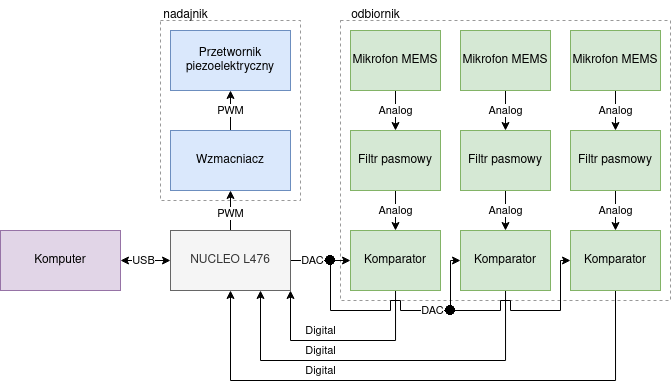
\includegraphics[width = 0.8\textwidth]{sonar_uml.png}
    \caption{Schemat blokowy urządzenia}
    \label{fig:uml}
\end{figure}

\section{Komunikacja}

\subsection{Wybór protokołu}

Wybrany został protokół UART, ze względu na to, że płytka deweloperska STM32 NUCLEO-L476RG 
z której skorzystano w projekcie posiada wbudowany konwerter UART$\rightarrow$~USB, 
co pozwala na skomunikowanie mikrokontrolera z komputerem bez dodatkowego sprzętu.

W celu uruchomienia sekwencji wykrywania obiektu operator powinien wysłać komendę przykładowo o nazwie "START". 
Komenda taka posiada swoje ID w formie pojedynczej cyfry, pozwoli to zmniejszyć ilość znaków zamieszczanych w ramce danych. 
Komunikacja tekstowa przede wszystkim pozwala na weryfikacje danych przez standardowy terminal tekstowy. 
Ramka danych rozpocznie się znakiem ,,X", pomoże to programowi odfiltrować tylko dane przeznaczone dla niego. ,,X" został wybrany ze względu na to, 
że znak ten na pewno nie będzie występował w treści wiadomości w żadnej postaci.
Wiadomość startu wraz z opcjonalnymi parametrami takimi jak ilość impulsów do wyemitowania czy próg czułości wykrywania sygnału wysłane są bajt po bajcie do urządzenia. 
Sonar rozpoznając znak początku ramki przechodzi dalej do odczytywania ID komendy oraz jej parametrów, po odebraniu całej wiadomości program zaczyna sekwencję pomiaru.
Następnie urządzenie wysyła do użytkownika odpowiedź, standardowo zaczyna znakiem rozpoznawczym a następnie zwraca numer ID komendy na którą ta wiadomość jest odpowiedzią,
status wykonania zadania, w formie kodów błędów, liczba wykrytych przecięć zer, oraz wartości liczników z każdego ze składowych pomiaru.
Dane będą przetwarzane przez operacje na obiektach typu {\tt string}. Pozwoli to na wycięcie odpowiednich wartości ze scalonej ramki wysłanej jako jeden długi ciąg znaków.

\subsection{Komputer \textrightarrow{} sonar}
Użytkownik systemu może wysłać z komputera instrukcję do wywołania całej sekwencji działania urządzenia. 
Ramka danych zaczyna się znakiem, który nie będzie nigdy występował w treści wiadomości, ułatwi to rozpoznanie wiadomości, 
następnie musi zostać podany numer komendy informujący sonar jaką czynność powinien wykonać oraz 
parametr określający warunki tej czynności. Informacje te zostały oddzielone znakiem spacji, a wiadomość zakończona znakiem końca lini i powrotu karetki.
Lista dostępnych komend została szerzej opisana w rozdziale \ref{chapter:specyfikacja}. 

\begin{figure}[!ht] %data in
    \centering
    \begin{tikztimingtable}[timing/wscale=4]
        \tikzset{% Environment Config
            timing/dslope=0.1,
            timing/.style={x=5ex,y=2ex},
            x=5ex,
            timing/rowdist=3ex,
            timing/name/.style={font=\sffamily\scriptsize},
            timing/d/text/.style={font=\sffamily\tiny},
        }
        \textcolor{black}{Instruction} & [black]
            Z 1D{X} 1D{}  1D{CMD\_ ID} 1D{} 1D{PAR}  1D{\textbackslash r \textbackslash n}  \\ %
        \textcolor{black}{Bytes} & [black]
            Z 1D{1}  1D{1}  1D{1}  1D{1}    1D{n}  1D{2}    \\ %
        %
        % there must NOT be an uncommented line before \extracode!
        %
        \extracode
            \tablerules
        %%  \tablegrid
        
        \begin{pgfonlayer}{background}
            \begin{scope}[semitransparent ,semithick]
                %\vertlines[darkgray,dotted]{1.0,3.0,...,23.0}
                \vertlines[gray,dotted]{4.0,8.0,...,\twidth}
            \end{scope}
        \end{pgfonlayer}
        \end{tikztimingtable}
        \caption{Ramka danych przychodzących}
        \label{fig:datain}
    \end{figure}

% \begin{figure}[!h]
%     \centering
%     \begin{tikztimingtable}[timing/wscale=4]
%         \tikzset{% Environment Config
%             timing/dslope=0.1,
%             timing/.style={x=5ex,y=2ex},
%             x=5ex,
%             timing/rowdist=3ex,
%             timing/name/.style={font=\sffamily\scriptsize},
%             timing/d/text/.style={font=\sffamily\tiny},
%         }
%         \busref*{FRAME}      & 2u 1d 2d 2u \\
%         \textcolor{black}{Instruction} & [black]
%             Z 1D{X}  1D{COM\_ID} 1D{CRC}    \\ %
%         \textcolor{black}{Bytes} & [black]
%             Z 1D{1}  1D{1}       1D{4}      \\ %
%         %
%         % there must NOT be an uncommented line before \extracode!
%         %
%         \extracode
%             \tablerules
%         %%  \tablegrid
        
%         \begin{pgfonlayer}{background}
%             \begin{scope}[semitransparent ,semithick]
%                 %\vertlines[darkgray,dotted]{1.0,3.0,...,23.0}
%                 \vertlines[gray,dotted]{4.0,8.0,...,\twidth}
%             \end{scope}
%         \end{pgfonlayer}
%         \end{tikztimingtable}
%     \end{figure}
    

\subsection{Sonar \textrightarrow{} komputer}

Sonar w odpowiedzi na instrukcję wysyła ramkę danych która również zaczyna się znakiem specjalnym. 
Tym razem jest to litera Y w celu rozróżnienia wiadomości wychodzących i przychodzących.
Następnie podawany jest status wykonania, 
liczba wykrytych przecięć sygnału z układem odniesienia oraz czasy wykrytych przecięć ze wszystkich odbiorników.
Podobnie jak w ramce z komendami przychodzącymi, wszystkie dane oddzielone są znakiem spacji a ramka zakończona znakiem końca linii oraz powrotu karetki.
Dodatkowo podczas pracy urządzenie zwraca informacje diagnostyczne o wykonanych działaniach, błędach i ostrzeżeniach.

\begin{figure}[!ht] %data out
\centering
\begin{tikztimingtable}[timing/wscale=4]
    \tikzset{% Environment Config
        timing/dslope=0.1,
        timing/.style={x=5ex,y=2ex},
        x=5ex,
        timing/rowdist=3ex,
        timing/name/.style={font=\sffamily\scriptsize},
        timing/d/text/.style={font=\sffamily\tiny},
    }
    \textcolor{black}{Instruction} & [black]
        Z 1D{X}  1D{ } 1D{STATUS} 1D{ } 1D{ZC\_NUM} 1D{ } 1D{D11} 1D{...} 1D{D33} 1D{\textbackslash r \textbackslash n}  \\ %
    \textcolor{black}{Bytes} & [black]
        Z 1D{1}  1D{1} 1D{1}      1D{1} 1D{1}       1D{1} 1D{32}   1D{...} 1D{32} 1D{2}      \\ %
    %
    % there must NOT be an uncommented line before \extracode!
    %
    \extracode
        \tablerules
    %%  \tablegrid
    
    \begin{pgfonlayer}{background}
        \begin{scope}[semitransparent ,semithick]
            %\vertlines[darkgray,dotted]{1.0,3.0,...,23.0}
            \vertlines[gray,dotted]{4.0,8.0,...,\twidth}
        \end{scope}
    \end{pgfonlayer}
    \end{tikztimingtable}
    \caption{Ramka danych wychodzących}
    \label{fig:dataout}
\end{figure}


\section{Konstrukcja układów elektronicznych sonaru}
Projekt bazuje na autorskiej płytce z obwodem drukowanym, który został zaprojektowany przy pomocy 
otwartoźródłowego narzędzia do projektowania elektroniki KiCad \cite{kicad}. 
Całe urządzenie składa się z płytki deweloperskiej oraz zaprojektowanego na cele pracy dyplomowej 
PCB (ang. Printed Circuit Board), które
jest podłączone do Nucleo w formie nakładki (ang. shield) poprzez listwy kołkowe.
Całą elektroniczną część urządzenia można podzielić na kilka bloków, ze względu na spełniane funkcje. 
Do bloków tych zaliczamy blok sekcji zasilania, blok nadawczy oraz blok odbiorczy. Ten ostatni zawiera zestaw filtrów sygnału odbieranego oraz komparatory progujące.

\subsection{Zasilanie}
Całe urządzenie zasilane jest z portu USB komputera, które jednocześnie służy do komunikacji. 
Przewód jest podłączony bezpośrednio do płytki deweloperskiej Nucleo, gdyż posiada ona już wbudowane złącze. 
Mimo, że płytka deweloperska posiada wyprowadzenia zarówno \unit[5]{V} jak i \unit[3,3]{V}, 
postanowiłem zaimplementować układ stabilizatora liniowego LM1117 obniżającego napięcie do \unit[3,3]{V} w celu lepszej izolacji 
zasilania układów analogowych od cyfrowych co powinno przełożyć się na mniejsze zakłócenia. 
Blisko jego wyprowadzeń zostały również umieszczone kondensatory konieczne do poprawnej stabilizacji, zgodnie z zaleceniami w nocie katalogowej \cite{ti:lm1117}
\begin{figure}[ht!]
    \centering
    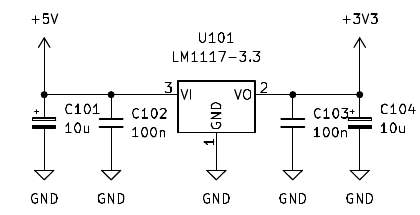
\includegraphics[width = 0.5\textwidth]{LDO.png}
    \caption{Stabilizator napięcia}
    \label{fig:ldo}
\end{figure}

\subsection{Nadajnik}
Rolę nadajnika pełni przetwornik piezoelektryczny BPU-1640T0AH12  o średnicy \unit[16]{mm} i częstotliwości rezonansowej \unit[40]{kHz}. 
która to jest poza spektrum słyszalnych dla człowieka częstotliwości wynoszącym \unit[16-20 000]{Hz} \cite{sluch}.
\begin{figure}[ht!]
    \centering
    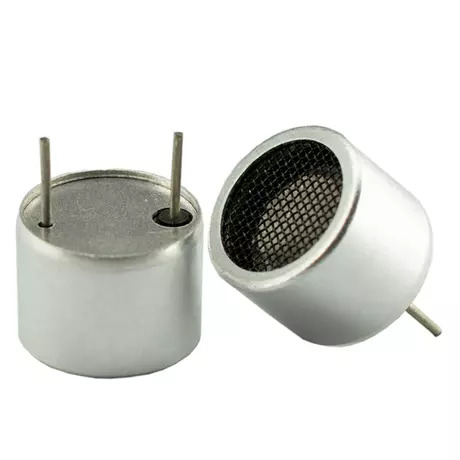
\includegraphics[width = 0.3\textwidth]{piezo.jpeg}
    \captionsource{Nadajnik piezoelektryczny}{\url{https://www.manorshi.com/}}
    \label{fig:piezo}
\end{figure}


\subsection{Wzmacniacz nadajnika}
W celu uzyskania mocnego sygnału ultradźwiękowego z przetwornika piezoelektrycznego zaprojektowano układ wzmacniający z transformatorem. 
Sygnał nadający częstotliwość wysyłany jest z mikroprocesora, następnie jest wzmacniany parą tranzystorów SS8550 oraz MMBT3904, razem tworzących układ Darlingtona, 
który zapewnia duże wzmocnienie prądowe sygnału i zachowuje krótkie czasy przełączania charakterystyczne dla tranzystorów bipolarnych.
Transformator w tym układzie służy do podniesienia napięcia które trafia na przetwornik, docelowo jest to nawet szczytowo \unit[80]{V} co sprawia, 
że sygnał jest bardzo mocny.
Układ posiada również zabezpieczenie przed zbyt długim czasem otwarcia tranzystora, sygnał jest przepuszczany przez kondensator C501 \ref{fig:piezo_amp}, 
co sprawia, że tylko szybkozmienne przebiegi są w stanie dotrzeć na bazę tranzystora Q502.
Zbyt długa ekspozycja transformatora na przepływ prądu mogłaby go narazić na przegrzanie.
Ze względu na indukcyjny charakter uzwojeń transformatora podczas szybkiej zmiany generowanego pola magnetycznego następuje 
konwersja tej energii do postaci prądu zwrotnego wyindukowanego na tej cewce. Aby uchronić się przed niepożądanym działaniem tego zjawiska, 
równolegle z uzwojeniem pierwotnym sprzężona jest dioda Schottkiego 1N5819WS, która pozwala zniwelować ten prąd.
Dodatkowo jako element ułatwiający pracę nad urządzeniem, dodany został LED, który emituje światło w trakcie przepływu prądu przez transformator.
\begin{figure}[ht!]
    \centering
    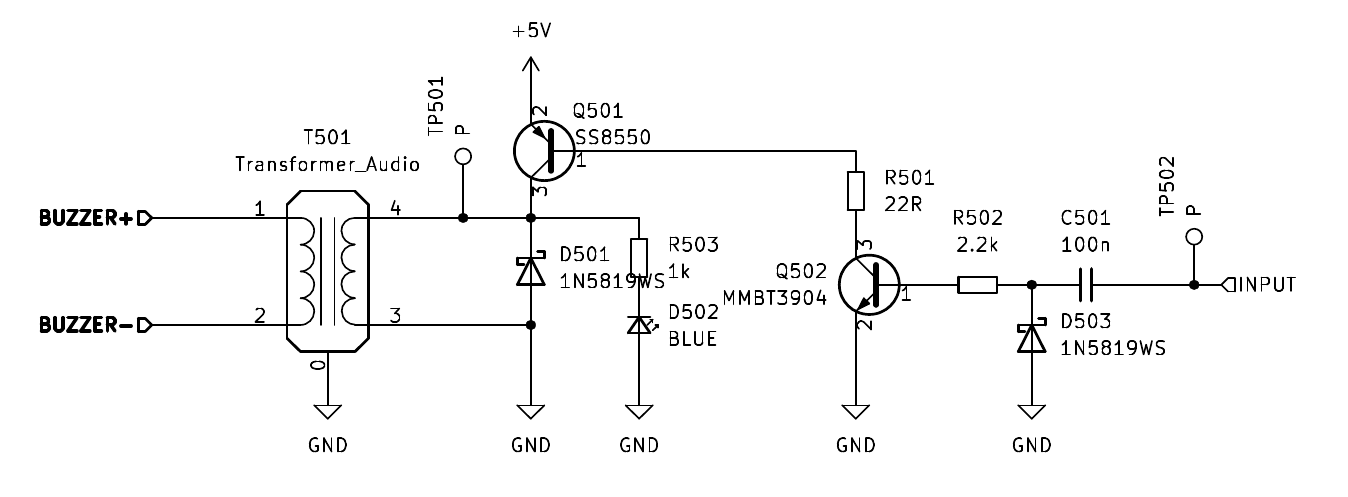
\includegraphics[width = \textwidth]{piezo_amp.png}
    \caption{Wzmacniacz sygnału nadajnika piezoelektrycznego}
    \label{fig:piezo_amp}
\end{figure}

\subsection{Filtry sygnału audio}

Przyjęto, że rolę odbiorników będą pełnić trzy dookólne mikrofony MEMS, które cechują się względnie liniową charakterystyką przenoszenia pasma. 
Dlatego też konieczne jest zastosowanie dla każdego z nich zestawu filtrów pasmowych, które przepuszczą nam tylko i wyłącznie częstotliwości bliskie częstotliwości 
sygnału jaki generuje przetwornik piezoelektryczny, a zablokują wszystkie niepożądane. 
Pojedynczy stopień filtra, dawałby na wyjściu zbyt niski zakres poziomu napięć, 
z tego powodu sygnał przechodzi przez 3 stopnie wzmacniaczy operacyjnych MCP6L04. Takie rozwiązanie zarówno filtruje sygnał i wzmacnia go.
\begin{figure}[ht!]
    \centering
    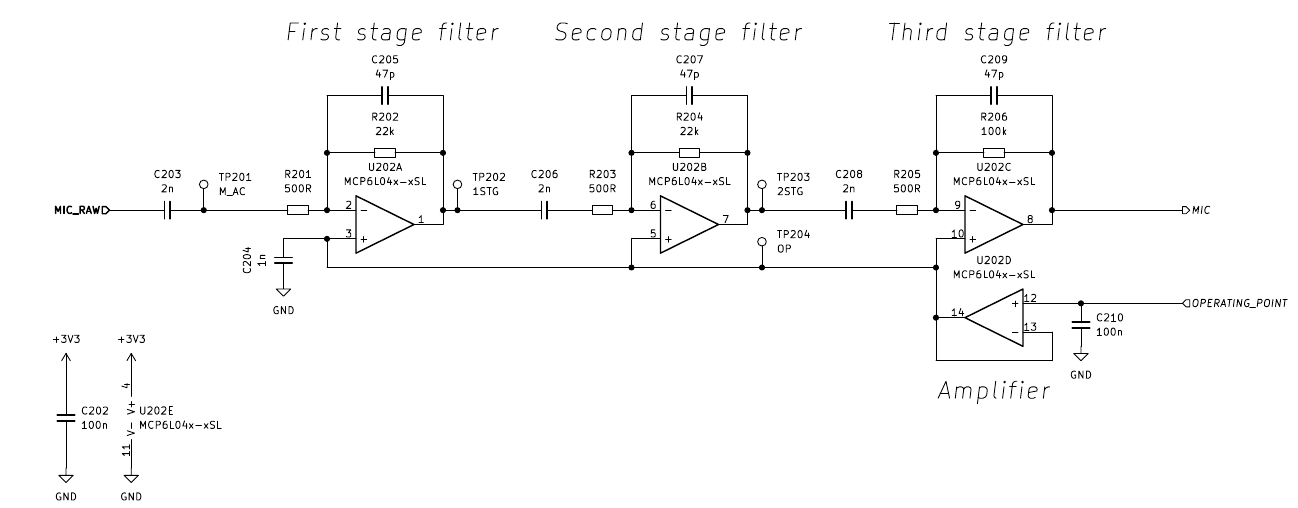
\includegraphics[width = \textwidth]{filter.png}
    \caption{Zestaw filtrów dla sygnału z mikrofonów}
    \label{fig:filter}
\end{figure}
\todo{zaktualizować rysunek}

Zazwyczaj układy analogowe oparte o wzmacniacze operacyjne zasilane są napięciem symetrycznym a sygnał przemienny oscyluje wokół potencjału masy. 
W tym wypadku ze względu na zakres napięciowy wejść mikroprocesora do zasilania wzmacniaczy operacyjnych 
zostało użyte pojedyncze napięcie \unit[3,3]{V} zamiast symetrycznego co oznacza, 
że chcąc uzyskać napięcie odniesienia w połowie zakresu zasilania należy ustalić je na poziomie \unit[1,65]{V}. 
Tę wartość ustala dzielnik napięcia z dwóch identycznych rezystorów,
a wzmacniacz operacyjny zwiększa wydajność prądową takiego źródła. 
\begin{figure}[ht!]
    \centering
    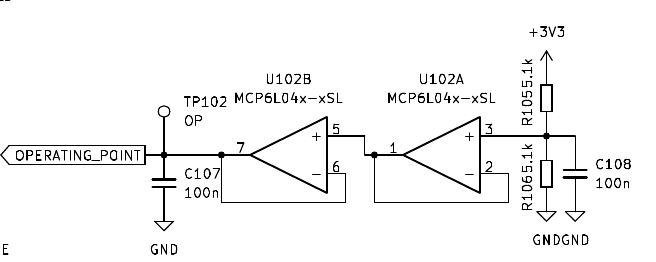
\includegraphics[width=0.7\textwidth]{op_point.png}
    \caption{Wzmacniacz prądowy napięcia odniesienia}
    \label{fig:op_point}
\end{figure}

\subsection{Progowanie sygnału}
Wejścia licznika reagują na zbocza sygnału cyfrowego, co oznacza, że analogowy sygnał z wyjścia filtra musi zostać przetworzony na stany logiczne.
Dokładna wartość napięcia nie jest potrzebna. Istotne są punkty przecięcia się sinusoidy z osią przebiegu.
Takie zadanie idealnie spełnia komparator LM239D \ref{fig:comparator}, próg od którego sygnał ma interpretować jako wysoki stan jest podawany w formie 
napięcia z przetwornika DAC mikrokontrolera dodatkowo wzmocnionego wzmacniaczem operacyjnym MCP6L04 \ref{fig:thereshold}.
Pozwala to na reagowanie tylko na falę dźwiękową o wystarczająco dużej amplitudzie, 
a po wykryciu mocnego sygnału wrócić z powrotem do poziomu napięcia odniesienia sygnału gdzie pomiar jest najdokładniejszy.

\begin{figure}[ht!]
    \centering
    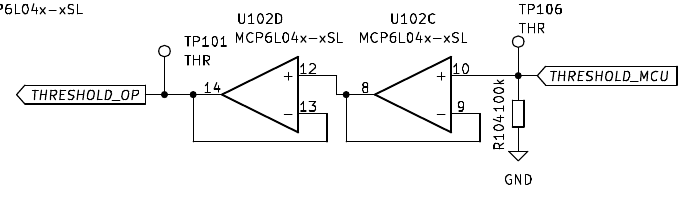
\includegraphics[width=0.7\textwidth]{thereshold.png}
    \caption{Wzmacniacz wartości progowej}
    \label{fig:thereshold}
\end{figure}

\begin{figure}[ht!]
    \centering
    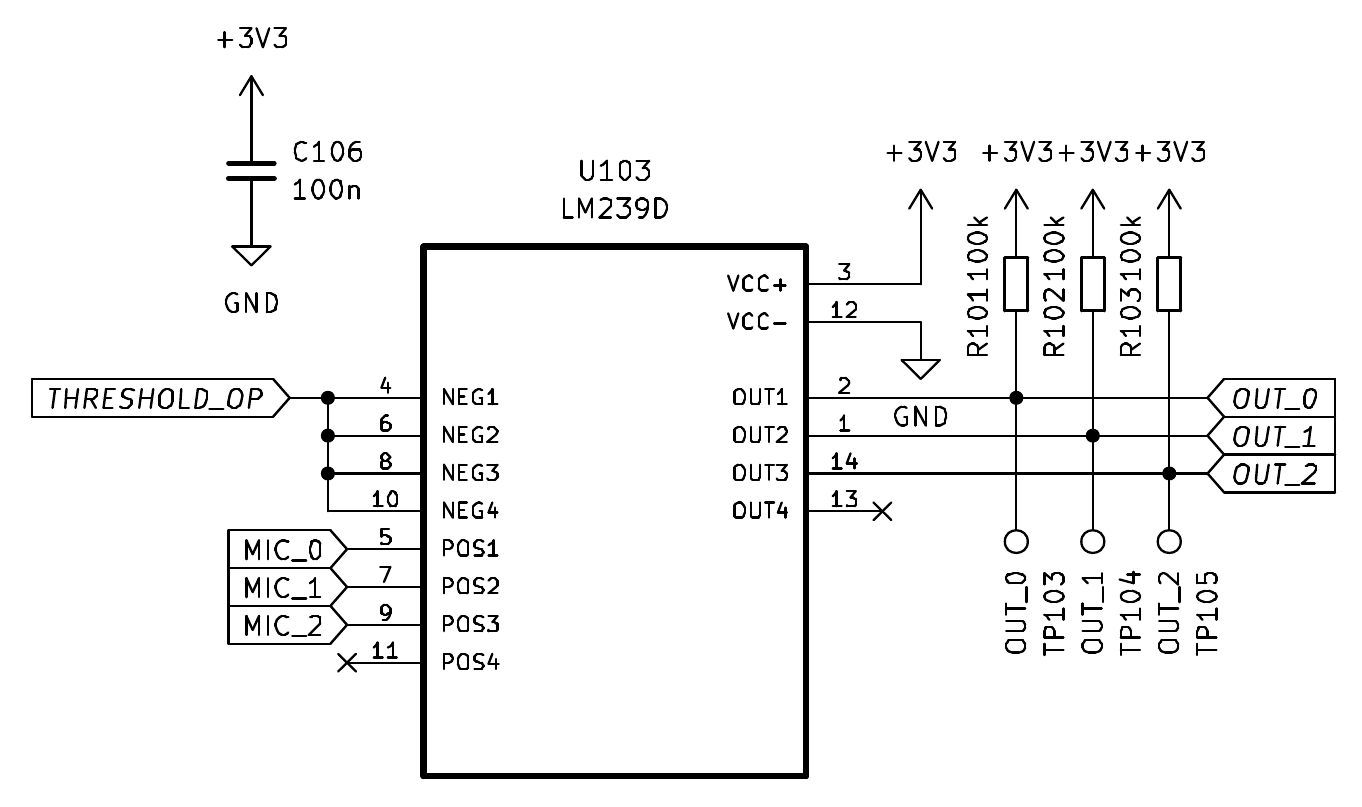
\includegraphics[width=0.7\textwidth]{comparator.png}
    \caption{Czterokanałowy komparator}
    \label{fig:comparator}
\end{figure}

\section{Konfiguracja mikrokontrolera}

Mikrokontroler użyty w projekcie to STM32L476 został on wybrany ze względu na odpowiednią liczbę liczników, przetworników i interfejsów komunikacji. 
Jego konfiguracja została przeprowadzona w programie STM32CUBEMX od firmy ST. 
Graficzny interfejs pozwala w łatwy sposób zmienić ustawienia peryferiów, 
taktowania zegarów systemowych czy nazwy zmiennych pomocniczych przydatnych na etapie programowania.
Gotowa konfiguracja wejść i wyjść została przedstawiona na rysunku nr \ref{fig:cube}, gdzie przyjęto następujące oznaczenia:

\begin{itemize}
    \item MIC\_0 -- pin do pomiaru sygnału z mikrofonu nr 0
    \item MIC\_1 -- pin do pomiaru sygnału z mikrofonu nr 1
    \item MIC\_2 -- pin do pomiaru sygnału z mikrofonu nr 2
    \item THR -- pin generujący napięcie progowania(thereshold) dla komparatora zewnętrznego 
    \item PIEZO -- pin sterujący przetwornikiem piezoelektrycznym 
    \item DBG\_LED -- pin obsługujący diodę diagnostyczną
    \item DBG\_BUT -- pin obsługujący przycisk diagnostyczny
\end{itemize}

\begin{figure}[ht!]
    \centering
    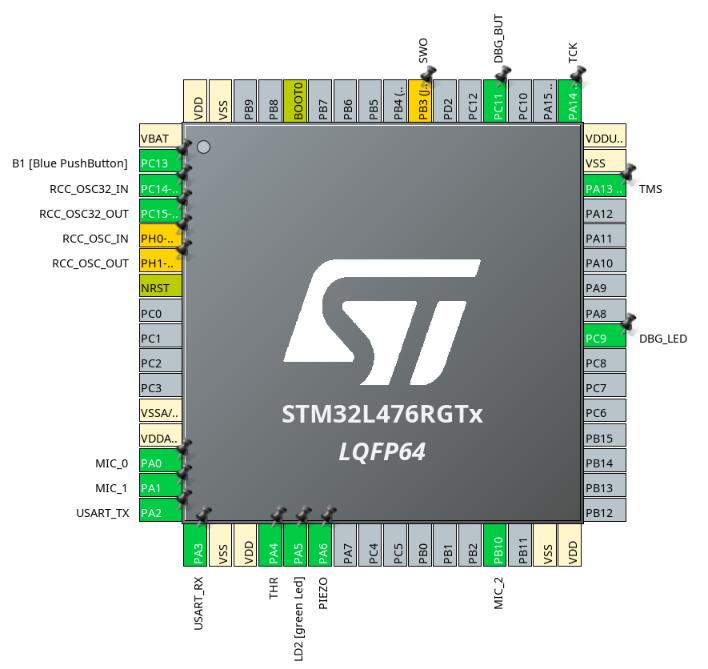
\includegraphics[width=0.7\textwidth]{cube.png}
    \caption{Konfiguracja pinów mikrokontrolera}
    \label{fig:cube}
\end{figure}
\todo{zaktualizować rysunek procka}

Piny odpowiedzialne za pomiary sygnału z mikrofonów zostały skonfigurowane jako wejścia 32 bitowego licznika TIM2 na osobnych kanałach. 
Została wykorzystana funkcja input capture, która wywołuje przerwanie za każdym razem jak wykryje zbocze rosnące lub opadające sygnału. 
W przerwaniu zaczytywana jest wartość licznika i przekazywana do bufora wiadomości.
Wyjście o nazwie THR zostało skonfigurowane jako przetwornik DAC, jego celem jest wygenerowanie napięcia, 
które jest progiem wykrycia sygnału dla komparatora \ref{fig:comparator}. Wartość ta podlega zmianie w trakcie pracy urządzenia, 
przez co użytkownik może dopasować czułość detektora, albo zwiększyć dokładność w trakcie trwania samego pomiaru.
Przetwornik piezoelektryczny sterowany jest sygnałem PWM, licznik TIM16 został skonfigurowany do pracy w PWM Generation z dodatkową opcją One Pulse Mode. 
Oznacza to, że licznik wykona dokładnie jeden okres sygnału o zadanych parametrach. 
W celu powtórzenia impulsu wyznaczoną przez użytkownika liczbę razy wykorzystany został rejestr RCR (Repetition Counter).
Elementy do debugowania zostały skonfigurowane jako zwykłe wyjście dla diody, oraz zwykłe wejście dla przycisku.

Taktowanie mikroprocesora zostało ustawiane na zalecaną maksymalną wartość \unit[80]{MHz}. 
Jak widać na rysunku nr \ref{fig:cube_clocks} z tej wartości korzystają również wszystkie użyte w projekcie peryferia. 
Co ma znaczenie podczas obliczania np częstotliwości sygnału PWM czy konwertowaniu wartości licznika na czas rzeczywisty.

\begin{figure}[ht!]
    \centering
    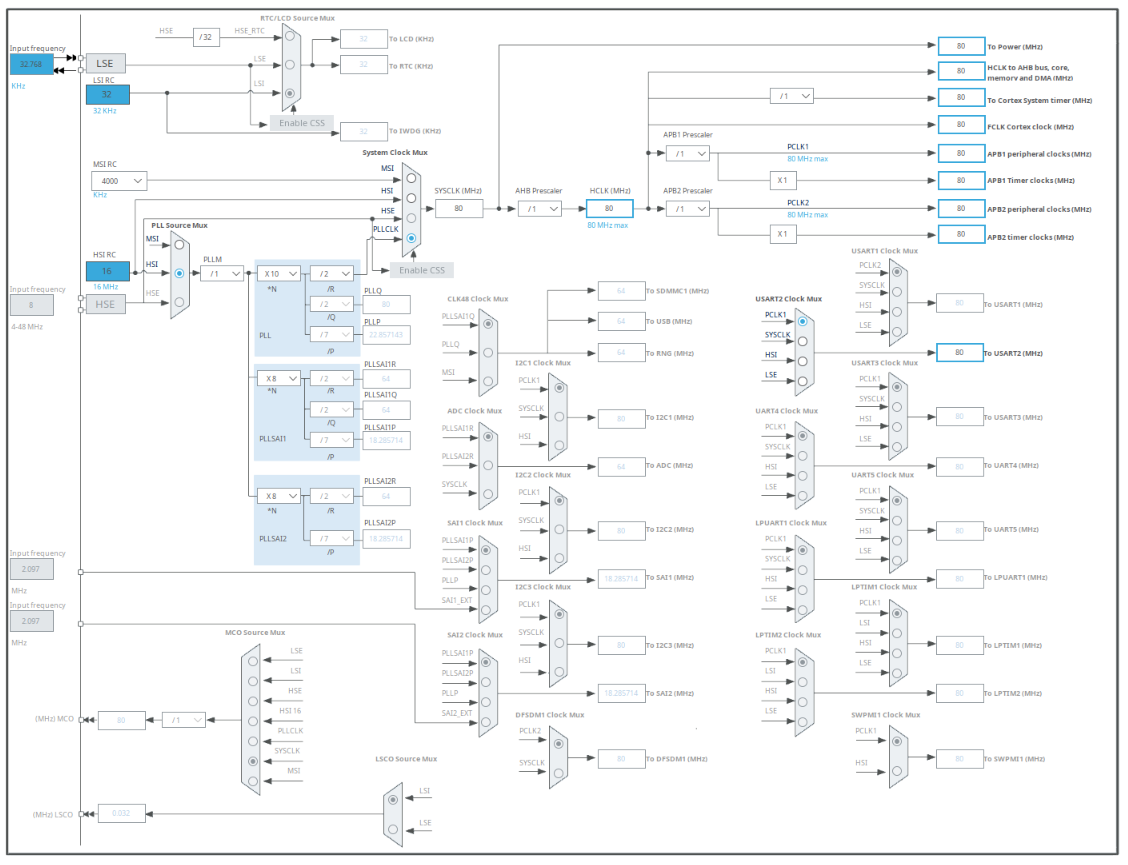
\includegraphics[width=\textwidth]{cube_clocks.png}
    \caption{Konfiguracja zegarów mikrokontrolera}
    \label{fig:cube_clocks}
\end{figure}

\clearpage
\section{Program}
Program w całości został napisany w języku C, korzystając z powłoki abstrakcji HAL od ST electronics. 
Większość funkcjonalności programu udało się zrealizować na przerwaniach systemowych oraz licznikach sprzętowych w celu maksymalizacji wydajności wykonywania operacji.
Pomiar przecięć sygnału  z układem odniesienia jest dokonywany poprzez czytanie wartości licznika w momencie wywołania przerwania zmianą stanu na jego wejściu.
Na wydruku \ref{lst:measure} przedstawiony został callback odpowiadający za pomiar czasów zmiany stanu.


\begin{listing}[tp]
    \begin{minted}[frame=single,framesep=10pt,fontsize=\scriptsize,linenos = true]{c}
void HAL_TIM_IC_CaptureCallback(TIM_HandleTypeDef *htim)
{
    switch (htim->Channel)
    {
    case HAL_TIM_ACTIVE_CHANNEL_1:
        active_channel = 1 - 1;
        zero_cross[0]++;
        set_timing_array(1, zero_cross[0], HAL_TIM_ReadCapturedValue(htim, TIM_CHANNEL_1));
        break;
    case HAL_TIM_ACTIVE_CHANNEL_2:
        active_channel = 2 - 1;
        zero_cross[1]++;
        set_timing_array(1, zero_cross[1], HAL_TIM_ReadCapturedValue(htim, TIM_CHANNEL_2));
        break;
    case HAL_TIM_ACTIVE_CHANNEL_3:
        active_channel = 3 - 1;
        zero_cross[2]++;
        set_timing_array(1, zero_cross[2], HAL_TIM_ReadCapturedValue(htim, TIM_CHANNEL_3));
        break;
    default:
        break;
    }
}
    \end{minted}
\SetupFloatingEnvironment{listing}{name= Wydruk}
\caption{Odbieranie przecięć przez zero}
\label{lst:measure}
\end{listing}

Wszystkie znaki przychodzące za pomocą peryferium UART są zapisywane w buforze, lecz dopiero kiedy napotkany zostanie znak końca linii, 
wykonywana jest operacja sprawdzenia poprawności danych w ciągu znaków. 
Odbieranie wiadomości w formie tekstowej opiera sie na funkcjach operujących na zmiennych typu \textit{string}. 
Funkcja \textit{sscanf} widoczna na wydruku \ref{lst:comm}  wyciąga z tekstowego typu danych liczby i konwertuje je na typ danych liczb całkowitych \textit{int}.
W ten sposób otrzymane dane przekazywane są do funkcji \textit{ExecCmd}, która wywołuje podaną w parametrach komendę z parametrami.
W celach diagnostycznych umieszczone zostały również linie kodu odpowiedzialne za wyświetlanie buforu po każdej odebranej wiadomości oraz komunikat błędu, 
jeżeli wiadomość ta nie spełnia kryteriów przyjętych podczas projektowania systemu komunikacji.

\begin{listing}[tp]
    \begin{minted}[frame=single,framesep=10pt,fontsize=\scriptsize,linenos = true]{c}
void MsgHandler()
{
    if (get_ready_to_send())
        SendResults();

    if (serial_available())
    {
        uint8_t c = serial_read();
        buff[buff_size] = c;
        buff_size++;
        if (c == '\n')
        {
            printf("Captured MSG: %s", buff);
            if (buff[0] == 'X' && sscanf(buff + 2, "%d %d", &cmdID, &param) == 2)
            {
                printf("MSG CmdId: %d, Param: %d \r\n", cmdID, param);
                ExecCmd(cmdID, param);
            }
            else
                printf("ERROR: MSG INVALID\r\n");
            memset(buff, 0, sizeof buff);
            buff_size = 0;
        }
    }
}
    \end{minted}
\SetupFloatingEnvironment{listing}{name= Wydruk}
\caption{Funkcja zarządzająca wiadomościami przychodzącymi i wychodzącymi}
\label{lst:comm}
\end{listing}


Po minięciu czasu zakończenia pomiaru, przerwanie wywołuje blok \ref{lst:send} odpowiedzialny za odesłanie wyników do komputera. Za pomocą funkcji \textit{printf}
dane wysyłane pojedynczo, a pakiet danych kończony jest znakiem końca linii po wysłaniu wszystkich danych zapisanych w buforze.

\begin{listing}[tp]
    \begin{minted}[frame=single,framesep=10pt,fontsize=\scriptsize,linenos = true]{c}
void SendResults()
{
    printf("Y 1 %c ", get_zero_cross(0));

    for (uint8_t i = 0; i < CHANNELS_NUM; i++)
    {
        for (uint8_t j = 0; i < get_pulse_count(); i++)
        {
            printf("%ld ", get_timing_array(i, j));
        }
    }
    printf("\r\n");
}
    \end{minted}
\SetupFloatingEnvironment{listing}{name= Wydruk}
\caption{Funkcja tworząca ramkę wiadomości wychodzącej}
\label{lst:send}
\end{listing}

